\item What is the minimum acceleration with which bar \( A \) (Fig. 1.22) should be shifted horizontally to keep bodies \( 1 \) and \( 2 \) stationary relative to the bar? The masses of the bodies are equal, and the coefficient of friction between the bar and the bodies is equal to \( k \). The masses of the pulley and the threads are negligible, the friction in the pulley is absent.
    \begin{center}
        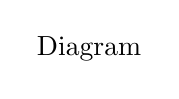
\begin{tikzpicture}
            \node at (0, 0) {Diagram};
        \end{tikzpicture}
    \end{center}